\documentclass[12pt,a4paper]{article}

\usepackage{fancyhdr}
\usepackage{graphicx}
\usepackage{placeins}
\usepackage{adjustbox}


\begin{document}

\pagestyle{fancy}
\fancyhf{}
\chead{Short summary report}

\begin{table}[t]
\centering
\caption {rnaQUAST metrics for assembled transcripts. In each row the best values are indicated with \textbf{bold}. For the transcript metrics (rows 4, 5, 6, 9, 13, 26, 27, 28) we highlighted the best \textbf{relative} values i.e. divided by the total number of transcripts in the corresponding assembly.}
\begin{adjustbox}{width=1\textwidth}
\small
\begin{tabular}{|l*{11}{|r}|}
\hline
\textbf{METRICS/TRANSCRIPTS}                            & \textbf{Trinity}       & \textbf{Trans-ABySS}   & \textbf{Oases}         & \textbf{SOAPdenovo-Trans} & \textbf{IDBA-Tran}     & \textbf{Bridger}       & \textbf{BinPacker}     & \textbf{Shannon}       & \textbf{rnaSPAdes}     & \textbf{SPAdes}        \\ \hline\hline
\multicolumn{11}{l}{\bf DATABASE METRICS}                                                 \\ \hline
Genes                                                   & 57992                  & 57992                  & 57992                  & 57992                  & 57992                  & 57992                  & 57992                  & 57992                  & 57992                  & 57992                  \\
Avg. number of exons per isoform                        & 5.971                  & 5.971                  & 5.971                  & 5.971                  & 5.971                  & 5.971                  & 5.971                  & 5.971                  & 5.971                  & 5.971                  \\ \hline
\multicolumn{11}{l}{\bf BASIC TRANSCRIPTS METRICS}                                        \\ \hline
Transcripts                                             & 97849                  & 213005                 & 178498                 & 131711                 & 78116                  & 83744                  & 12291                  & 84456                  & 206133                 & 93814                  \\
Transcripts $>$ 500 bp                                  & 42497                  & 58213                  & 114976                 & 24636                  & 31500                  & 33578                  & \textbf{11834}         & 27820                  & 32697                  & 25204                  \\
Transcripts $>$ 1000 bp                                 & 27785                  & 32866                  & 83530                  & 13418                  & 14196                  & 20560                  & \textbf{10862}         & 15007                  & 18629                  & 13245                  \\ \hline
\multicolumn{11}{l}{\bf ALIGNMENT METRICS}                                                \\ \hline
Aligned                                                 & 97647                  & 212044                 & 177747                 & 130789                 & 77999                  & 83546                  & 12274                  & \textbf{84373}         & 203335                 & 87567                  \\
Uniquely aligned                                        & 94046                  & 204947                 & 161313                 & 128896                 & 77059                  & 79021                  & 10437                  & 82753                  & 199122                 & 81873                  \\
Multiply aligned                                        & 549                    & 1999                   & 1048                   & 1263                   & 407                    & 404                    & 19                     & 421                    & 1496                   & 1707                   \\
Unaligned                                               & 202                    & 961                    & 751                    & 922                    & 117                    & 198                    & 17                     & \textbf{83}            & 2798                   & 6247                   \\ \hline
\multicolumn{11}{l}{\bf ALIGNMENT METRICS FOR NON-MISASSEMBLED TRANSCRIPTS}               \\ \hline
Avg. aligned fraction                                   & 0.984                  & 0.984                  & 0.937                  & \textbf{0.995}         & 0.993                  & 0.977                  & 0.929                  & 0.994                  & 0.987                  & 0.984                  \\
Avg. alignment length                                   & 1143.492               & 578.881                & 1500.776               & 482.257                & 725.58                 & 929.857                & \textbf{3072.898}      & 703.748                & 476.176                & 649.419                \\
Avg. mismatches per transcript                          & 1.684                  & 0.769                  & 2.311                  & \textbf{0.468}         & 0.866                  & 1.43                   & 3.755                  & 0.583                  & 1.15                   & 0.951                  \\ \hline
\multicolumn{11}{l}{\bf ALIGNMENT METRICS FOR MISASSEMBLED (CHIMERIC) TRANSCRIPTS}          \\ \hline
Misassemblies                                           & 1066                   & 3253                   & 11194                  & \textbf{94}            & 134                    & 1844                   & 1436                   & 381                    & 908                    & 1206                   \\ \hline
\multicolumn{11}{l}{\bf ASSEMBLY COMPLETENESS (SENSITIVITY)}                              \\ \hline
Database coverage                                       & 0.161                  & \textbf{0.188}         & 0.176                  & 0.143                  & 0.136                  & 0.131                  & 0.048                  & 0.116                  & 0.159                  & 0.126                  \\
50\%-assembled genes                                    & 8947                   & \textbf{9467}          & 9166                   & 8582                   & 7964                   & 7837                   & 3054                   & 6519                   & 9283                   & 8232                   \\
95\%-assembled genes                                    & 3486                   & 3292                   & \textbf{3579}          & 2667                   & 710                    & 2492                   & 1353                   & 1502                   & 3363                   & 2650                   \\
50\%-covered genes                                      & 10329                  & 11000                  & 10167                  & 10251                  & 10120                  & 9192                   & 3115                   & 8262                   & \textbf{11020}         & 9329                   \\
95\%-covered genes                                      & 4299                   & 4434                   & \textbf{4451}          & 3404                   & 1744                   & 2981                   & 1415                   & 2188                   & 4217                   & 3034                   \\
50\%-assembled isoforms                                 & 12623                  & \textbf{15475}         & 15176                  & 9979                   & 9764                   & 9616                   & 3794                   & 8309                   & 11326                  & 9031                   \\
95\%-assembled isoforms                                 & 4065                   & 3575                   & \textbf{4330}          & 2749                   & 714                    & 2736                   & 1523                   & 1631                   & 3535                   & 2654                   \\
50\%-covered isoforms                                   & 14765                  & \textbf{19493}         & 17208                  & 12503                  & 13253                  & 11421                  & 3874                   & 10900                  & 13922                  & 10517                  \\
95\%-covered isoforms                                   & 4991                   & 4943                   & \textbf{5457}          & 3512                   & 1755                   & 3246                   & 1591                   & 2369                   & 4440                   & 3039                   \\
Mean isoform coverage                                   & 0.515                  & 0.461                  & 0.551                  & 0.385                  & 0.451                  & 0.444                  & \textbf{0.719}         & 0.473                  & 0.403                  & 0.439                  \\
Mean isoform assembly                                   & 0.462                  & 0.401                  & 0.504                  & 0.335                  & 0.382                  & 0.399                  & \textbf{0.707}         & 0.402                  & 0.354                  & 0.398                  \\ \hline
\multicolumn{11}{l}{\bf GeneMarkS-T METRICS}                                              \\ \hline
Predicted genes                                         & 30009                  & 43585                  & \textbf{73686}         & 16066                  & 23174                  & 21088                  & 8375                   & 23879                  & 21429                  & 15644                  \\ \hline
\multicolumn{11}{l}{\bf ASSEMBLY SPECIFICITY}                                             \\ \hline
50\%-matched                                            & 51949                  & 99617                  & 109483                 & 55068                  & 43657                  & 40396                  & \textbf{9462}          & 56036                  & 56981                  & 33929                  \\
95\%-matched                                            & 33810                  & 70234                  & 57036                  & 46001                  & 36242                  & 28362                  & 4836                   & \textbf{48039}         & 40135                  & 25755                  \\
Unannotated                                             & 33696                  & 90840                  & 35015                  & 60913                  & 24679                  & 29047                  & \textbf{202}           & 23378                  & 128667                 & 42074                  \\
Mean fraction of transcript matched                     & 0.524                  & 0.462                  & 0.623                  & 0.419                  & 0.559                  & 0.492                  & \textbf{0.83}          & 0.658                  & 0.277                  & 0.379                  \\ \hline
\end{tabular}
\end{adjustbox}
\end{table}

\FloatBarrier
\clearpage
\lfoot{generated by rnaQUAST}

\begin{figure}[t]
\centering
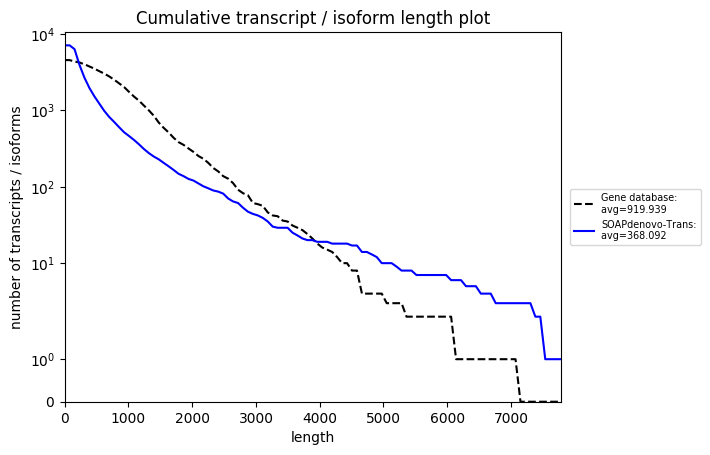
\includegraphics[width = \linewidth]{/mnt/dessertlocal/projects/transcriptome_assembly/review/evaluation/rna-quast/ebov_hsa_23h/comparison_output/transcript_length.png}
\caption{Plot showing cumulative transcript length distribution. Each point represents the number of transcripts in the assembly with the corresponding length or longer; black dashed line corresponds to the database isoforms; the plot is given in logarithmic scale.}
\end{figure}
\FloatBarrier
\clearpage


\begin{figure}[t]
\centering
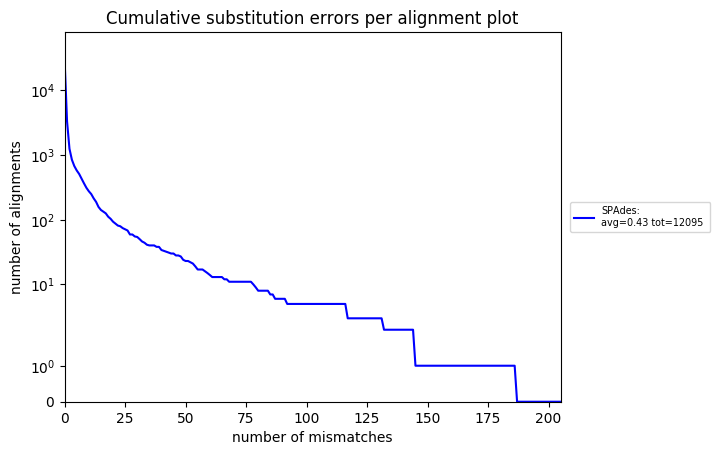
\includegraphics[width = \linewidth]{/mnt/dessertlocal/projects/transcriptome_assembly/review/evaluation/rna-quast/ebov_hsa_23h/comparison_output/mismatch_rate.png}
\caption{Plot showing cumulative substitution errors per alignment distribution. Each point represents the number of alignments with the corresponding number of mismatches or greater; the plot is given in logarithmic scale.}
\end{figure}
\FloatBarrier
\clearpage


\begin{figure}[t]
\centering
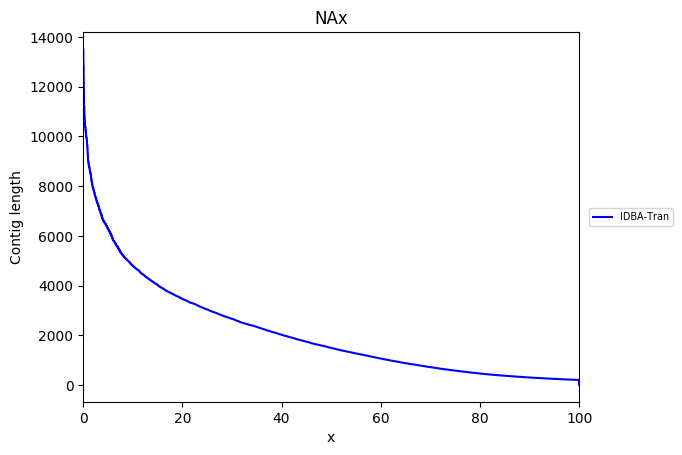
\includegraphics[width = \linewidth]{/mnt/dessertlocal/projects/transcriptome_assembly/review/evaluation/rna-quast/ebov_hsa_23h/comparison_output/NAx.png}
\caption{Nx plot for transcripts. Nx is a maximal number $N$, such that the total length of all transcripts longer than $N$ bp is at least $x\%$ of the total length of all transcripts.}
\end{figure}
\FloatBarrier
\clearpage


\begin{figure}[t]
\centering
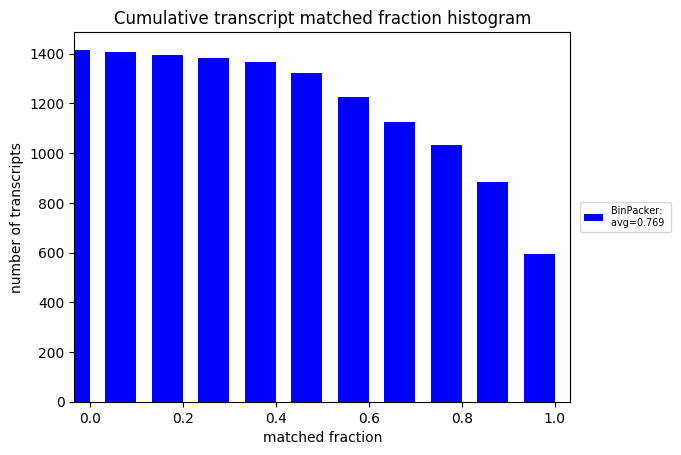
\includegraphics[width = \linewidth]{/mnt/dessertlocal/projects/transcriptome_assembly/review/evaluation/rna-quast/ebov_hsa_23h/comparison_output/x-matched.png}
\caption{Plot showing cumulative transcript match histogram. Each bar represents the number of transcripts with matched fraction equal to or greater than the value on $x$ axis; transcript matched fraction is calculated as the number of its bases covering an isoform divided by the transcript length.}
\end{figure}
\FloatBarrier
\clearpage


\begin{figure}[t]
\centering
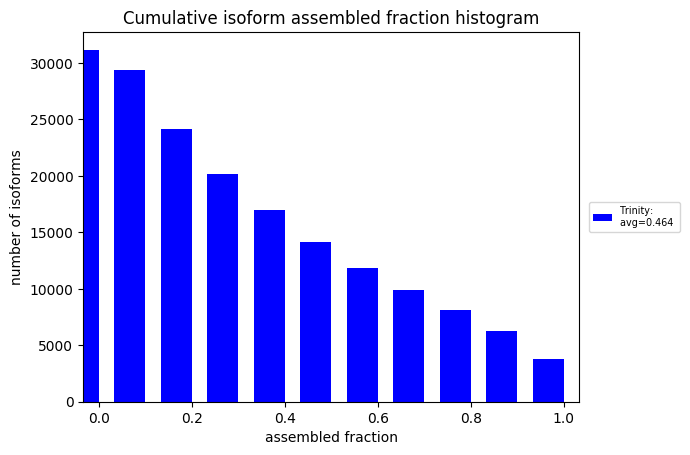
\includegraphics[width = \linewidth]{/mnt/dessertlocal/projects/transcriptome_assembly/review/evaluation/rna-quast/ebov_hsa_23h/comparison_output/x-assembled.png}
\caption{Plot showing cumulative isoform assembly histogram. Each bar represents the number of isoforms with assembled fraction equal to or greater than the value on $x$ axis; isoform assembled fraction is calculated as the maximum number of captured by single assembled transcript bases divided by the total isoform length.}
\end{figure}
\FloatBarrier
\clearpage


\begin{figure}[t]
\centering
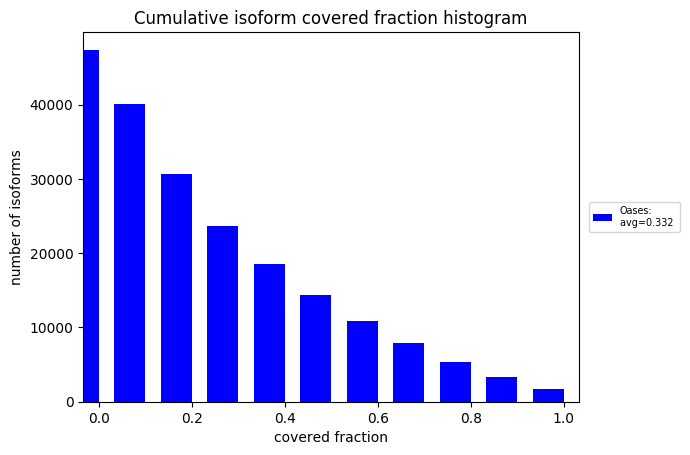
\includegraphics[width = \linewidth]{/mnt/dessertlocal/projects/transcriptome_assembly/review/evaluation/rna-quast/ebov_hsa_23h/comparison_output/x-covered.png}
\caption{Plot showing cumulative isoform coverage histogram. Each bar represents the number of isoforms with covered fraction equal to or greater than the value on $x$ axis; isoform covered fraction is calculated as the number of covered bases (by all transcripts in the assembly) divided by the total isoform length.}
\end{figure}
\FloatBarrier
\clearpage


\end{document}
